\section{Versuch}
\subsection{Versuchsaufbau}
Die benutzten Werkzeuge sind der PtIr-Draht, ein Seitenschneider, eine Zange, eine Pinzette, die Proben HOPG und Gold, sowie das Rastertunnelmikroskop mit einer Abdichtung in der eine Lupe mit zehnfacher Verstärkung verbaut ist.

\noindent Die in Kapitel zwei beschriebene Schwierigkeit der Vibrationen wird durch einen Schwingungsdämpfenden Tisch der zusätzlich auf vier dämpfenden isolierungs Füßen steht, glöst. Der Tisch ist aus Granit um eine möglichst schwere Grundfläche zu gewährleisten. Die Füße sind aus Gummi um ein Verrutschen der Vorrichtung zu verhindern und sind intern mit Federn ausgestattet um die letzten Schwingungen zu dämpfen. Auf dem Tisch ist die Messvorrichtung installiert.

\noindent Ein Aufbau ist in Abbildung \ref{fig:Aufbau1} dargestellt. 

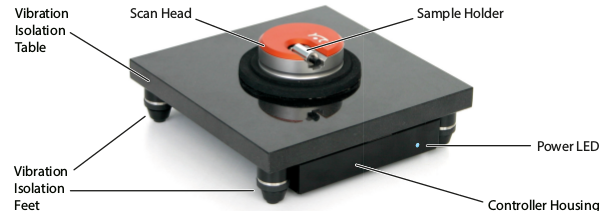
\includegraphics{Aufbau1.png}
\begin{figure}
	\centering
		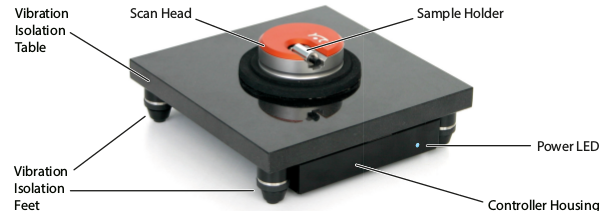
\includegraphics[width=0.5\textwidth]{Aufbau1}
	\caption{Rastertunnelmikroskop}
	\label{fig:Aufbau1}
\end{figure}

\noindent Einen genaueren Einblick in die Messvorrichtung wird in Abbildung \ref{fig:Aufbau2} gegeben.

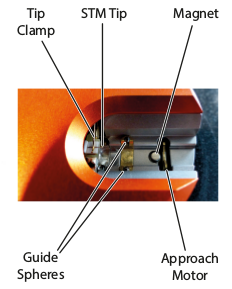
\includegraphics{Aufbau2.png}
\begin{figure}
	\centering
		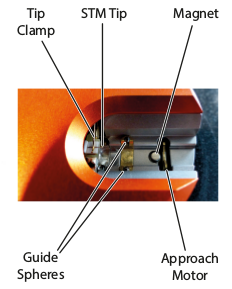
\includegraphics[width=0.5\textwidth]{Aufbau2}
	\caption{Messvorrichtung}
	\label{fig:Aufbau2}
\end{figure}

\noindent Durch den Magnet wird die Probenhalterung, die an ihrer Spitze selbst magnetisiert ist um die Probe, die auf einer kreisförmigen Metallscheibe liegt, an ihren Ort fixiert. Die Spitze wird unter einen Bügel in eine dafür vorgesehene Furche gelegt und dort festgehalten. Die magnetischen Kugeln, sowie der Motor verschieben die Probe an den gewünschten Ort.

\subsection{Versuchsdurchführung}
Zunächst wurden die Werkzeuge mit 2-Propanol gereinigt. Mit der Zange wurde ein Stück des Drahts festgehalten und mit dem Seitenschneider wurde dann (Nahezu parallel zur Zange gehalten) eine Spitze aus dem Draht gerissen. Zuletzt wurde die Spitze auf die richtige Größe geschnitten und mit der Pinzette unter den Bügel gelegt.

\noindent Daraufhin wurde eine Probe genommen (Wegen der thermisch isolierten Halterung am Ende, ist das Anfassen mit der Hand möglich) und in die Messvorrichtung gelegt. Die Abdichtung wurde darauf gestellt.

\noindent Der Rest der Durchführung geschah mit dem Programm ''Nanosurf NaioSTM''.

\includegraphics{Programm.png}
\begin{figure}
	\centering
		\includegraphics[width=0.5\textwidth]{Programm}
	\caption{Programminterface: Nanosurf NaioSTM}
	\label{fig:Programm}
\end{figure}

\noindent Als Erstes wurde über den ''more''-Button das Menü für die SPM-Parameter geöffnet und unter ''Imaging'' -> ''Imaging Modes'' -> ''Scan Mode'', ''Scan Fw. \& Bw.'' ausgewählt, sodass die Spitze in einem Schlangenförmigenweg die Probe abtastet.

\noindent Mit ''Advance'' bzw. ''Approach'' konnte die Spitze an die Probe gefahren werden. Nachdem die richtigen Parameter unter ''Parameters'' eingestellt wurden, musste noch eine Spannung (\(50\)mV) an die Spitze angelegt werden. Dies geschah durch die Einstellung unter ''Mode Properties''.